\documentclass{tufte-handout}

\usepackage{style}

\begin{document}

\tma{04} % TMA number

\section{Part A}


%Question 8
\begin{question}

    Question 8 from section B

Let \( R \) be the ring \( \Z[\sqrt{-13}] \)

\qpart

\[ A = \{ s + t\sqrt{-13} : s,t \in \Z, s - t \equiv 0\pmod{7} \} \]

As \( s = t\pmod{7} \) there eisits an integer \( k \) such that,
\[ s = t + 7k \]
Hence,
\begin{align*}
s + t\sqrt{-13} &= (t + 7k) + t\sqrt{-13} \\[8pt]
&= t(1 + \sqrt{-13}) + 7k\\[8pt]
\stext{So}
A \langle 7, 1 + \sqrt{-13} \rangle
\end{align*} 

By \textup{Definition 2.1 HB Chapter 17 p94},

To Show \( A \) is ideal, it must be closed under multiplication by any \( r \in R \).
So we need the product of the generator and \( \sqrt{-13} \) to stay in \( A \).

\begin{align*}
\sqrt{-13}(1 + \sqrt{-13}) &= \sqrt{-13} -13\\[8pt]
\stext{since} -13 &\equiv 1\pmod{7} \\[8pt]
-13 &= 1 -14\\[8pt]
\sqrt{-13} -13 &= (\sqrt{-13} + 1) - 14\\[8pt]
&= (\sqrt{-13} + 1) + 7(-2)
\end{align*}

Since \( (\sqrt{-13} + 1) \in A \) and \( 14 = 2(7) \in A \) it follows that \( A \) 
is closed under multiplication by any element of \( R \) and hence is an ideal.

\vspace{3cm}

\qpart

\[ B = \{ u + v\sqrt{-13} : u,v \in \Z, u + v \equiv 0\pmod{7} \} \]

As \( u = -v\pmod{7} \) there eisits an integer \( k \) such that, 
\[ u = -v + 7k \] 

Hence, 
\begin{align*} 
    u + v\sqrt{-13} &= (-v + 7k) + v\sqrt{-13} \\[8pt] 
    &= v(-1 + \sqrt{-13}) + 7k\\[8pt] 
    \stext{So} 
    B \langle 7, -1 + \sqrt{-13} \rangle
\stext{because \( -1 \) is a unit in \( \Z[\sqrt{-13}] \), therefore we can multiply the second generator by \( -1 \) and it will still generate the same ideal.}
    B \langle 7, 1 - \sqrt{-13} \rangle
\end{align*}

Hence,

\begin{align*}
A & \langle 7, 1 + \sqrt{-13} \rangle \\[8pt]
\stext{and}
B & \langle 7, 1 - \sqrt{-13} \rangle\\[8pt]
\stext{By \textup{Lemma 3.9 HB Chapter 17 p97}, the product of two ideals \(A\) and \( B \)}
AB & \langle 7\cdot 7, 7(1 - \sqrt{-13}), 7(1 + \sqrt{-13}), (1 + \sqrt{-13})(1 - \sqrt{-13}) \rangle \\[8pt] 
& \langle 49, 7(1 - \sqrt{-13}), 7(1 + \sqrt{-13}), 14 \rangle\\[8pt]
\stext{Since the \( \hcf(14, 49) = 7 \) and \( 7(1 - \sqrt{-13}) \) and \( 7(1 + \sqrt{-13}) \) are multiples of \( 7 \) and,}
7 &= 49 -3(14) \in AB\\[8pt]
7 &\subseteq AB\\[8pt]
\stext{hence}
AB & \langle 7 \rangle
\end{align*}



\end{question}


\end{question}

%Question 9
Question 9 from section B
\begin{question}

\[ B_{d}((0,0),1), B_{d}[(0,0),1], \text{ and } S_{s}((0,0),1)   \]

By \textup{Defintion 2.6 HB Chapter 14 p 72}

\qpart

The open ball on metric 
\[ d((a_{1},a_{2}),(b_{1},b_{2})) = 6|b_{1} - a_{1}| + |b_{2} - a_{2}| \]

is given by
\begin{align*}
B_{d}((0,0),1) &= \{ (x,y) \in \R^{2} : d((x,y),(0,0)) < 1 \} \\[8pt]
&= \{ (x,y) \in \R^{2} : 6|x - 0| + |y - 0| < 1 \} \\[8pt]
&= \{ (x,y) \in \R^{2} : 6|x| + |y| < 1 \}      
\end{align*}

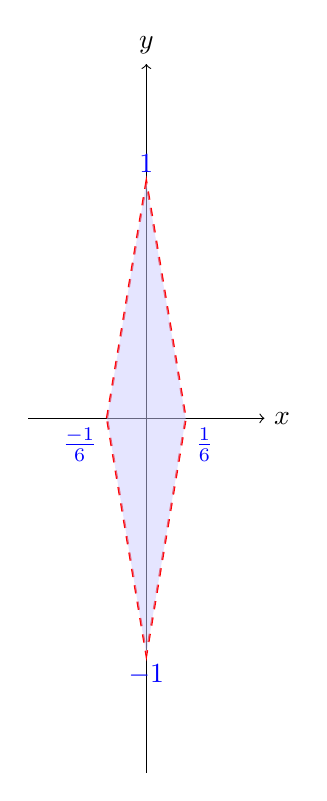
\begin{tikzpicture}[scale=3]
    %axis
    \draw[->] (-0.5,0) -- (0.5,0) node[right] {$x$};
    \draw[->] (0,-1.5) -- (0,1.5) node[above] {$y$};

    %boundry (dashes)
    \draw[thick, dashed, red] (-1/6,0) -- (0,1) -- (1/6,0) -- (0,-1) -- cycle;
    \fill[blue!20,opacity=0.5] (-1/6,0) -- (0,1) -- (1/6,0) -- (0,-1) -- cycle;

    %labels
    \node[blue, below left] at (-1/6,0) {$\frac{-1}{6}$};
    \node[blue, below right] at (1/6,0) {$\frac{1}{6}$};
    \node[blue, above] at (0,1) {$1$};
    \node[blue, below] at (0,-1) {$-1$};
\end{tikzpicture}

The closed ball on metric
\[ d((a_{1},a_{2}),(b_{1},b_{2})) = 6|b_{1} - a_{1}| + |b_{2} - a_{2}| \]

is given by
\begin{align*}
B_{d}[(0,0),1] &= \{ (x,y) \in \R^{2} : d((x,y),(0,0)) \leq 1 \} \\[8pt]
&= \{ (x,y) \in \R^{2} : 6|x - 0| + |y - 0| \leq 1 \} \\[8pt]
&= \{ (x,y) \in \R^{2} : 6|x| + |y| \leq 1 \}      
\end{align*}

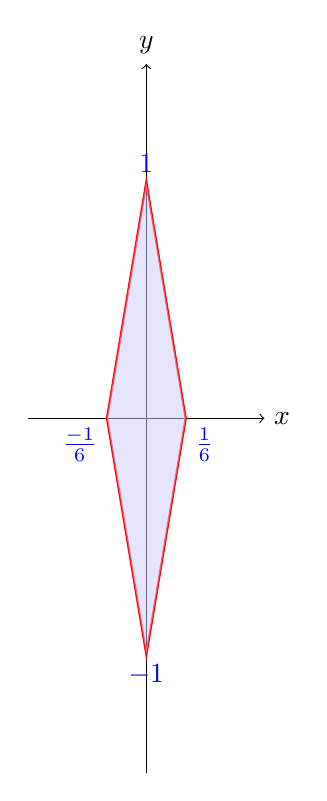
\begin{tikzpicture}[scale=3]
    %axis
    \draw[->] (-0.5,0) -- (0.5,0) node[right] {$x$};
    \draw[->] (0,-1.5) -- (0,1.5) node[above] {$y$};

    %boundry (solid)
    \draw[thick, red] (-1/6,0) -- (0,1) -- (1/6,0) -- (0,-1) -- cycle;
    \fill[blue!20,opacity=0.5] (-1/6,0) -- (0,1) -- (1/6,0) -- (0,-1) -- cycle;

    %labels
    \node[blue, below left] at (-1/6,0) {$\frac{-1}{6}$};
    \node[blue, below right] at (1/6,0) {$\frac{1}{6}$};
    \node[blue, above] at (0,1) {$1$};
    \node[blue, below] at (0,-1) {$-1$};
\end{tikzpicture}

Thh sphere on metric
\[ d((a_{1},a_{2}),(b_{1},b_{2})) = 6|b_{1} - a_{1}| + |b_{2} - a_{2}| \] is given by
\begin{align*}
S_{s}((0,0),1) &= \{ (x,y) \in \R^{2} : d((x,y),(0,0)) = 1 \} \\[8pt]
&= \{ (x,y) \in \R^{2} : 6|x - 0| + |y - 0| = 1 \} \\[8pt]
&= \{ (x,y) \in \R^{2} : 6|x| + |y| = 1 \}      
\end{align*}

\begin{tikzpicture}[scale=3]
    %axis
    \draw[->] (-0.5,0) -- (0.5,0) node[right] {$x$};
    \draw[->] (0,-1.5) -- (0,1.5) node[above] {$y$};

    %boundry (solid)
    \draw[thick, red] (-1/6,0) -- (0,1) -- (1/6,0) -- (0,-1) -- cycle;

    %labels
    \node[blue, below left] at (-1/6,0) {$\frac{-1}{6}$};
    \node[blue, below right] at (1/6,0) {$\frac{1}{6}$};
    \node[blue, above] at (0,1) {$1$};
    \node[blue, below] at (0,-1) {$-1$};
\end{tikzpicture}

\qpart

The open ball on metric
\[ d((a_{1},a_{2}),(b_{1},b_{2})) = (|b_{1} - a_{1}|^{4}  + |b_{2} - a_{2}|^4)^{\frac{1}{4}} \]

is given by
\begin{align*}
B_{d}((0,0),1) &= \{ (x,y) \in \R^{2} : d((x,y),(0,0)) < 1 \} \\[8pt]
&= \{ (x,y) \in \R^{2} : (|x - 0|^{4} + |y - 0|^{4})^{\frac{1}{4}} < 1 \} \\[8pt]
&= \{ (x,y) \in \R^{2} : (|x|^{4} + |y|^{4})^{\frac{1}{4}} < 1 \}      
\end{align*}

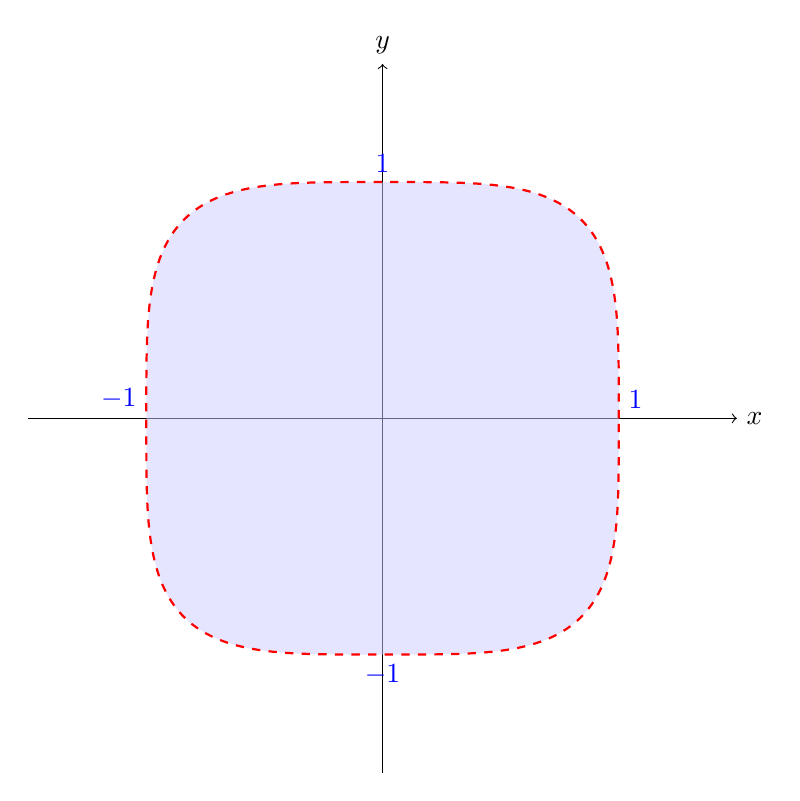
\begin{tikzpicture}[scale=3]
    % axes
    \draw[->] (-1.5,0) -- (1.5,0) node[right] {$x$};
    \draw[->] (0,-1.5) -- (0,1.5) node[above] {$y$};

    % L^4 unit ball boundary: |x|^4 + |y|^4 = 1 (parametric, robust)
    % r(t) = (|cos t|^4 + |sin t|^4)^(-1/4)
    \fill[blue!20,opacity=0.5]
      plot[domain=0:360,samples=240,smooth]
      ({cos(\x)*(abs(cos(\x))^4 + abs(sin(\x))^4)^(-1/4)},
       {sin(\x)*(abs(cos(\x))^4 + abs(sin(\x))^4)^(-1/4)}) -- cycle;

    \draw[thick, dashed, red]
      plot[domain=0:360,samples=240,smooth]
      ({cos(\x)*(abs(cos(\x))^4 + abs(sin(\x))^4)^(-1/4)},
       {sin(\x)*(abs(cos(\x))^4 + abs(sin(\x))^4)^(-1/4)});

    % labels
    \node[blue, above right] at (1,0) {$1$};
    \node[blue, above left] at (-1,0) {$-1$};
    \node[blue, above] at (0,1) {$1$};
    \node[blue, below] at (0,-1) {$-1$};
\end{tikzpicture}

The closed ball on metric
\[ d((a_{1},a_{2}),(b_{1},b_{2})) = (|b_{1} - a_{1}|^{4}  + |b_{2} - a_{2}|^4)^{\frac{1}{4}} \] is given by
\begin{align*}
B_{d}[(0,0),1] &= \{ (x,y) \in \R^{2} : d((x,y),(0,0)) \leq 1 \} \\[8pt]
&= \{ (x,y) \in \R^{2} : (|x - 0|^{4} + |y - 0|^{4})^{\frac{1}{4}} \leq 1 \} \\[8pt]
&= \{ (x,y) \in \R^{2} : (|x|^{4} + |y|^{4})^{\frac{1}{4}} \leq 1 \}      
\end{align*}    

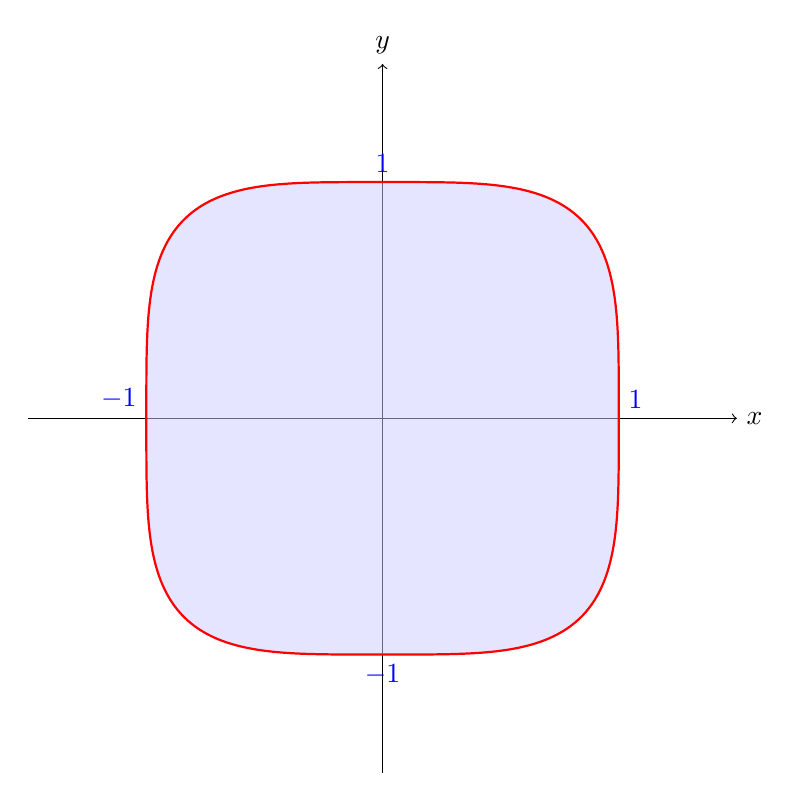
\begin{tikzpicture}[scale=3]
    % axes
    \draw[->] (-1.5,0) -- (1.5,0) node[right] {$x$};
    \draw[->] (0,-1.5) -- (0,1.5) node[above] {$y$};

    % fill the closed ball
    \fill[blue!20,opacity=0.5]
      plot[domain=0:360,samples=240,smooth]
      ({cos(\x)*(abs(cos(\x))^4 + abs(sin(\x))^4)^(-1/4)},
       {sin(\x)*(abs(cos(\x))^4 + abs(sin(\x))^4)^(-1/4)}) -- cycle;

    % boundary (solid)
    \draw[thick, red]
      plot[domain=0:360,samples=240,smooth]
      ({cos(\x)*(abs(cos(\x))^4 + abs(sin(\x))^4)^(-1/4)},
       {sin(\x)*(abs(cos(\x))^4 + abs(sin(\x))^4)^(-1/4)});

    % labels
    \node[blue, above right] at (1,0) {$1$};
    \node[blue, above left] at (-1,0) {$-1$};
    \node[blue, above] at (0,1) {$1$};
    \node[blue, below] at (0,-1) {$-1$};
\end{tikzpicture}

The sphere on metric
\[ d((a_{1},a_{2}),(b_{1},b_{2})) = (|b_{1} - a_{1}|^{4}  + |b_{2} - a_{2}|^4)^{\frac{1}{4}} \] is given by
\begin{align*}
S_{s}((0,0),1) &= \{ (x,y) \in \R^{2} : d((x,y),(0,0)) = 1 \} \\[8pt]
&= \{ (x,y) \in \R^{2} : (|x - 0|^{4} + |y - 0|^{4})^{\frac{1}{4}} = 1 \} \\[8pt]       
&= \{ (x,y) \in \R^{2} : (|x|^{4} + |y|^{4})^{\frac{1}{4}} = 1 \}
\end{align*}        

\begin{tikzpicture}[scale=3]
    % axes
    \draw[->] (-1.5,0) -- (1.5,0) node[right] {$x$};
    \draw[->] (0,-1.5) -- (0,1.5) node[above] {$y$};

    % boundary only (sphere)
    \draw[thick, red]
      plot[domain=0:360,samples=240,smooth]
      ({cos(\x)*(abs(cos(\x))^4 + abs(sin(\x))^4)^(-1/4)},
       {sin(\x)*(abs(cos(\x))^4 + abs(sin(\x))^4)^(-1/4)});

    % labels
    \node[blue, above right] at (1,0) {$1$};
    \node[blue, above left] at (-1,0) {$-1$};
    \node[blue, above] at (0,1) {$1$};
    \node[blue, below] at (0,-1) {$-1$};
\end{tikzpicture}

\qpart

The open ball on metric
\[ d((a_{1},a_{2}),(b_{1},b_{2})) = d_{0}(a_{1},b_{1}) + 6|b_{2} - a_{2}| \]

is given by
\begin{align*}
S_{s}((0,0),1) &= \{ (x,y) \in \R^{2} : d((x,y),(0,0)) < 1 \} \\[8pt]
&= \{ (x,y) \in \R^{2} : d_{0}(x,0) + 6|y - 0| < 1 \} \\[8pt]
&= \{ (x,y) \in \R^{2} : d_{0}(x,0) + 6|y| < 1 \}   
\end{align*}

\begin{tikzpicture}[scale=3]
    %axis
    \draw[->] (-0.5,0) -- (0.5,0) node[right] {$x$};
    \draw[->] (0,-1) -- (0,1) node[above] {$y$};

    %boundry (solid)
    \draw[dashed, thick, red] (0,-1/6) -- (0,1/6);
    
    %labels
    \node[blue, right] at (0,1/6) {$\frac{1}{6}$};
    \node[blue, right] at (0,-1/6) {$\frac{-1}{6}$};
  
\end{tikzpicture}

The closed ball on metric
\[ d((a_{1},a_{2}),(b_{1},b_{2})) = d_{0}(a_{1},b_{1}) + 6|b_{2} - a_{2}| \] is given by
\begin{align*}
B_{d}[(0,0),1] &= \{ (x,y) \in \R^{2} : d((x,y),(0,0)) \leq 1 \} \\[8pt]
&= \{ (x,y) \in \R^{2} : d_{0}(x,0) + 6|y - 0| \leq 1 \} \\[8pt]
&= \{ (x,y) \in \R^{2} : d_{0}(x,0) + 6|y| \leq 1 \}   
\end{align*}    

\begin{tikzpicture}[scale=3]
    %axis
    \draw[->] (-0.5,0) -- (0.5,0) node[right] {$x$};
    \draw[->] (0,-1) -- (0,1) node[above] {$y$};

    %boundry (solid)
    \draw[thick, red] (0,-1/6) -- (0,1/6);
    \fill[blue!20,opacity=0.5] (0,-1/6) -- (0,1/6) -- cycle;
    
    %labels
    \node[blue, right] at (0,1/6) {$\frac{1}{6}$};
    \node[blue, right] at (0,-1/6) {$\frac{-1}{6}$};

\end{tikzpicture}

The sphere on metric
\[ d((a_{1},a_{2}),(b_{1},b_{2})) = d_{0}(a_{1},b_{1}) + 6|b_{2} - a_{2}| \] is given by
\begin{align*}
S_{s}((0,0),1) &= \{ (x,y) \in \R^{2} : d((x,y),(0,0)) = 1 \} \\[8pt]
&= \{ (x,y) \in \R^{2} : d_{0}(x,0) + 6|y - 0| = 1 \} \\[8pt]
&= \{ (x,y) \in \R^{2} : d_{0}(x,0) + 6|y| = 1 \}   
\end{align*}

\begin{tikzpicture}[scale=3]
    %axis
    \draw[->] (-0.5,0) -- (0.5,0) node[right] {$x$};
    \draw[->] (0,-1) -- (0,1) node[above] {$y$};

    %boundry (solid)
    \draw[thick, red] (0,-1/6) -- (0,1/6);
    
    %labels
    \node[blue, right] at (0,1/6) {$\frac{1}{6}$};
    \node[blue, right] at (0,-1/6) {$\frac{-1}{6}$};
\end{tikzpicture}



\end{question}

\end{document}